\subsection*{\underline{Probability Distributions:}}
\paragraph{}We have three distributions, one for classical particles (Maxwell-Boltzmann) and two for undistinguishable particles (Fermi-Dirac for fermions and Bose-Einstein for bosons). Their equations are the following:
\begin{gather}
    P(E)=\frac{1}{e^{\beta(E -E_f)}+1} \qquad \text{Fermi--Dirac Dist.}\\
    P(E)=\frac{1}{e^{\beta(E -\mu)}-1} \qquad \text{Bose--Einstein Dist.}\\
    P(E)=\frac{1}{e^{\beta(E -\mu)}} \qquad \text{Maxwell--Boltzmann Dist.}\\
    \text{Where $\beta=\frac{1}{k_B T}$}
\end{gather}
\paragraph{}The plots of these distributions for different temperatures:
\begin{center}
    \frame{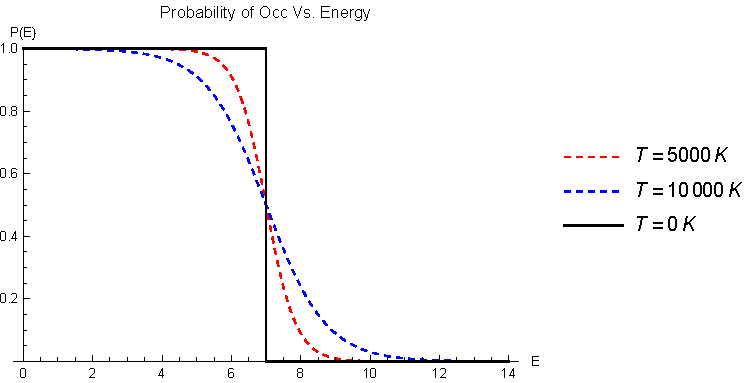
\includegraphics[width=10cm]{./figures/pt1.pdf}}\\
    \textbf{Figure 1:} Fermi--Dirac Dist. when $E_f=7eV$. For fermions\\
\end{center}
\par
\begin{center}
    \frame{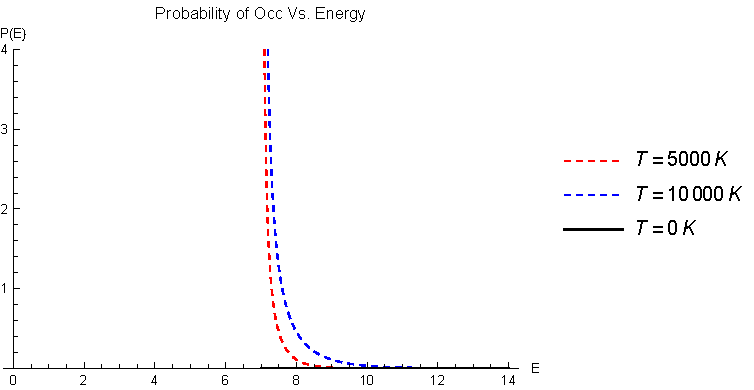
\includegraphics[width=10cm]{./figures/pt2.pdf}}\\
    \textbf{Figure 2:} Bose--Einstein Dist. when $\mu=7eV$. For bosons\\
\end{center}
\begin{center}
    \frame{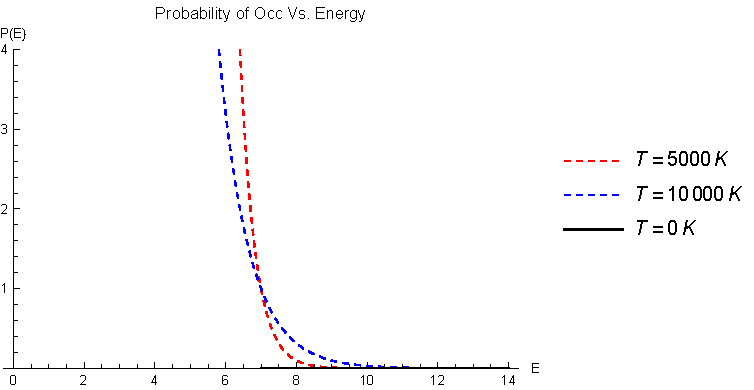
\includegraphics[width=10cm]{./figures/pt3.pdf}}\\
    \textbf{Figure 3:} Maxwell--Boltzmann Dist. when $\mu=7eV$. For bosons\\
\end{center}